\graphicspath{{png/}}

\section{Демонстрация работы программы}

Каркасная визуализация поверхности. В программе пользователь может задать цвет каркаса, выбрать, отрисовывать ли контрольные точки.

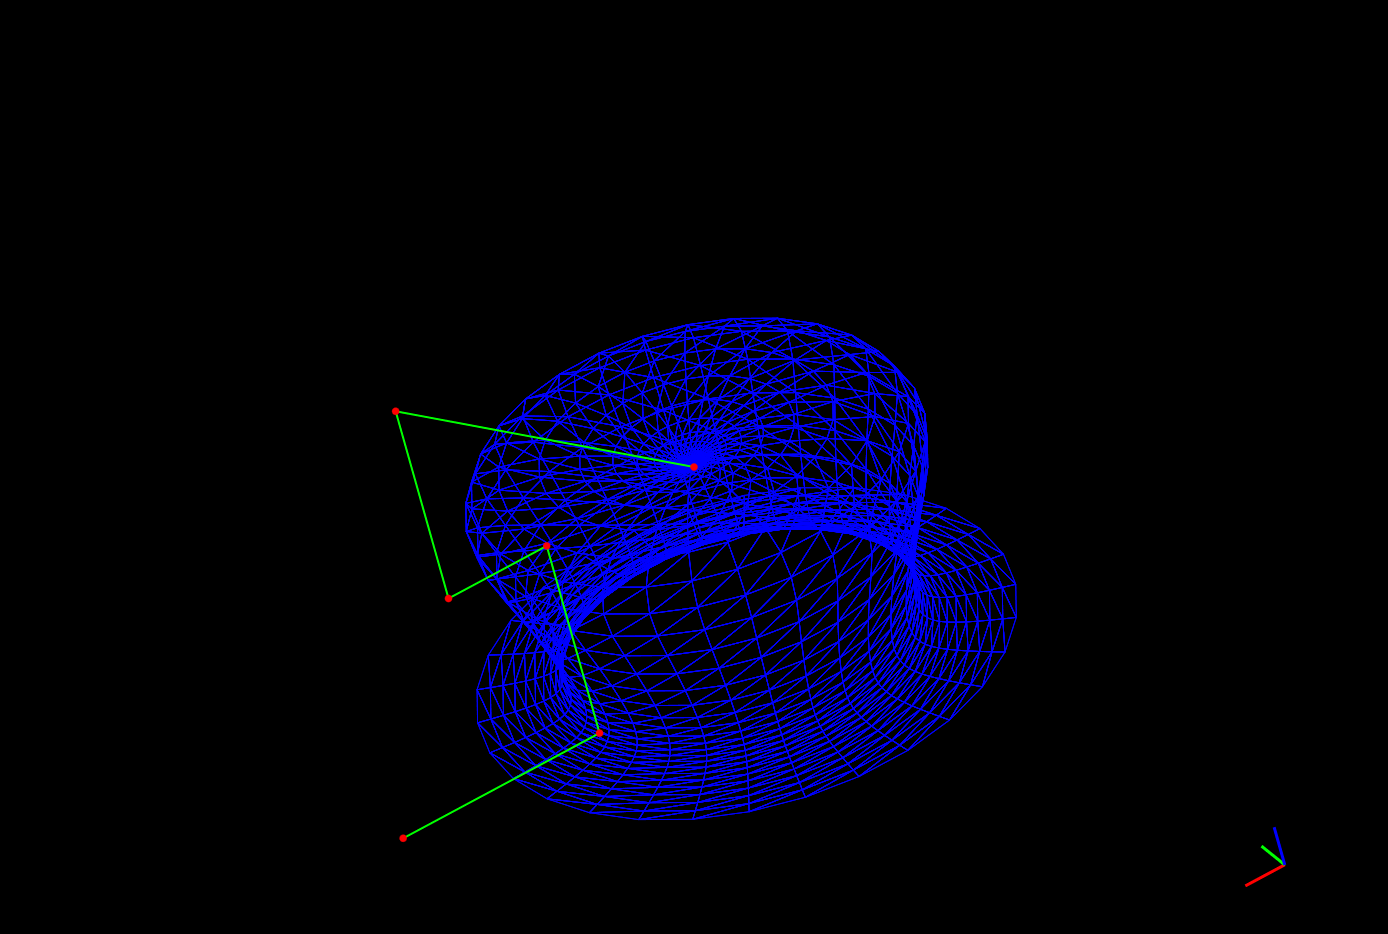
\includegraphics[scale=0.16]{img1}
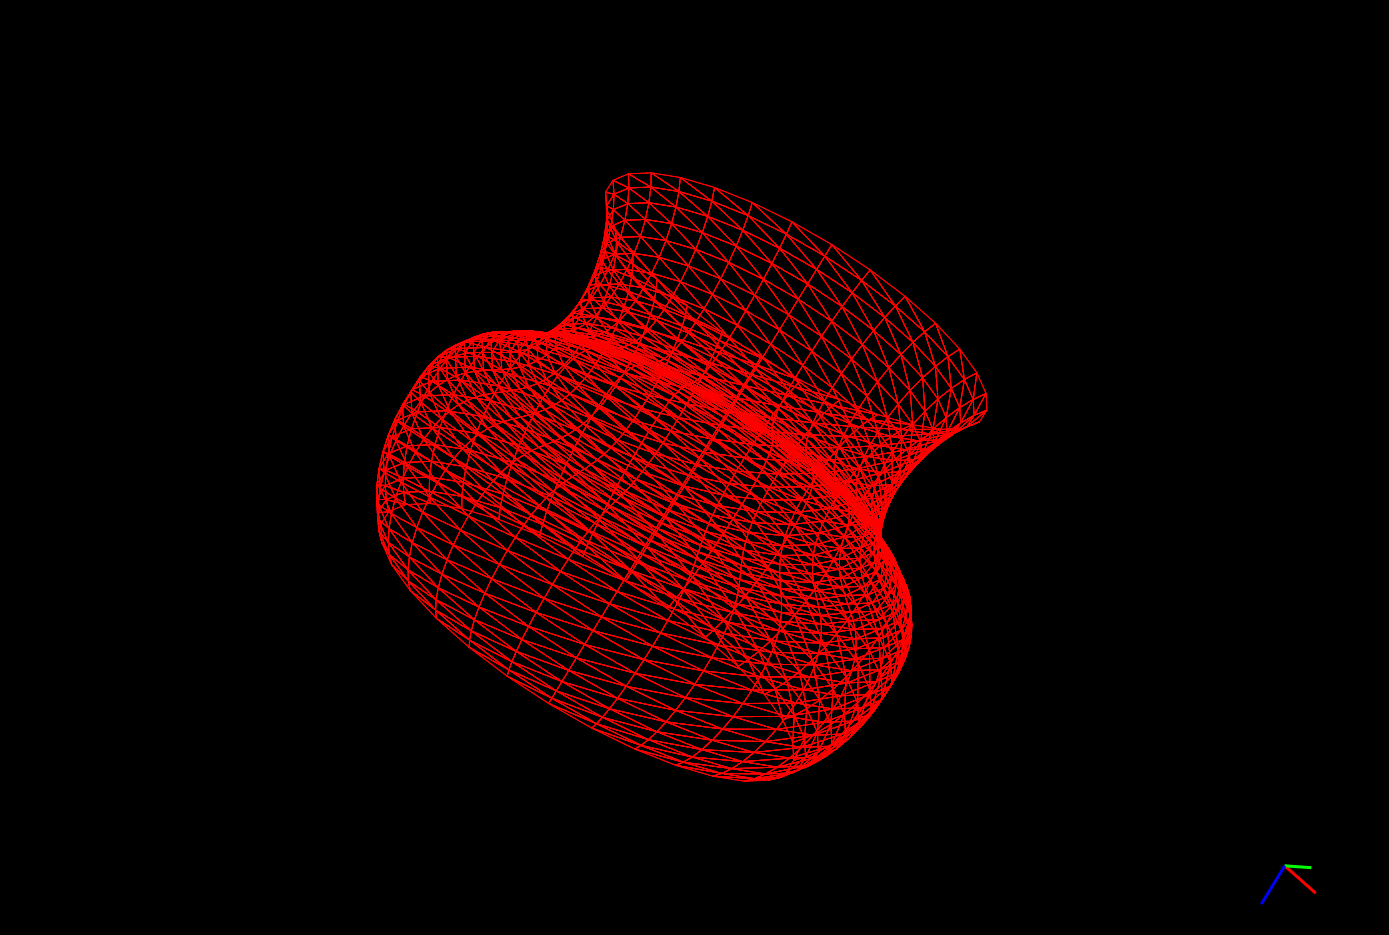
\includegraphics[scale=0.16]{img2}

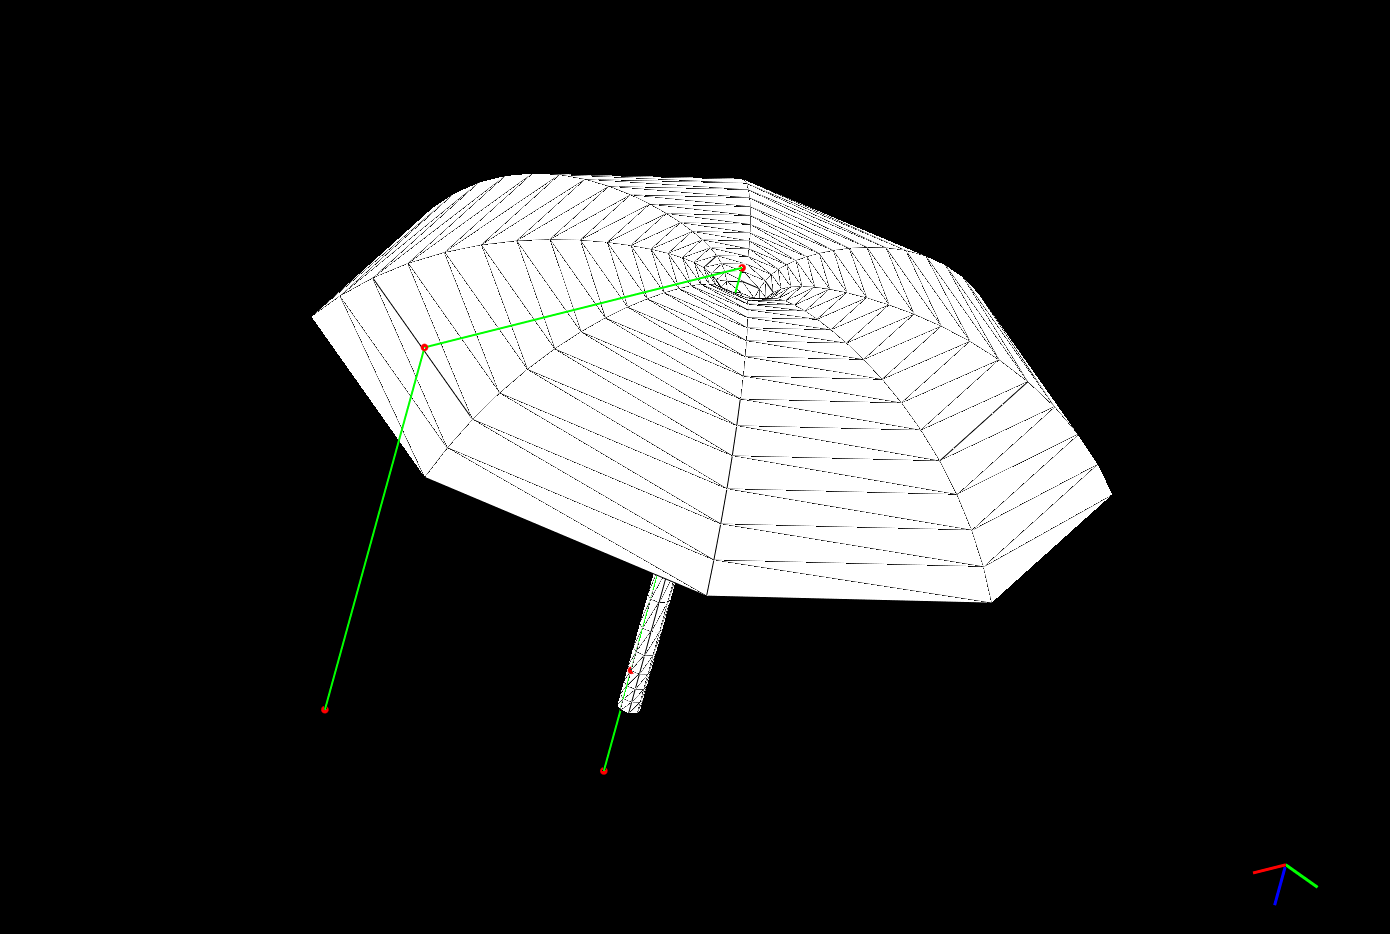
\includegraphics[scale=0.16]{img3}
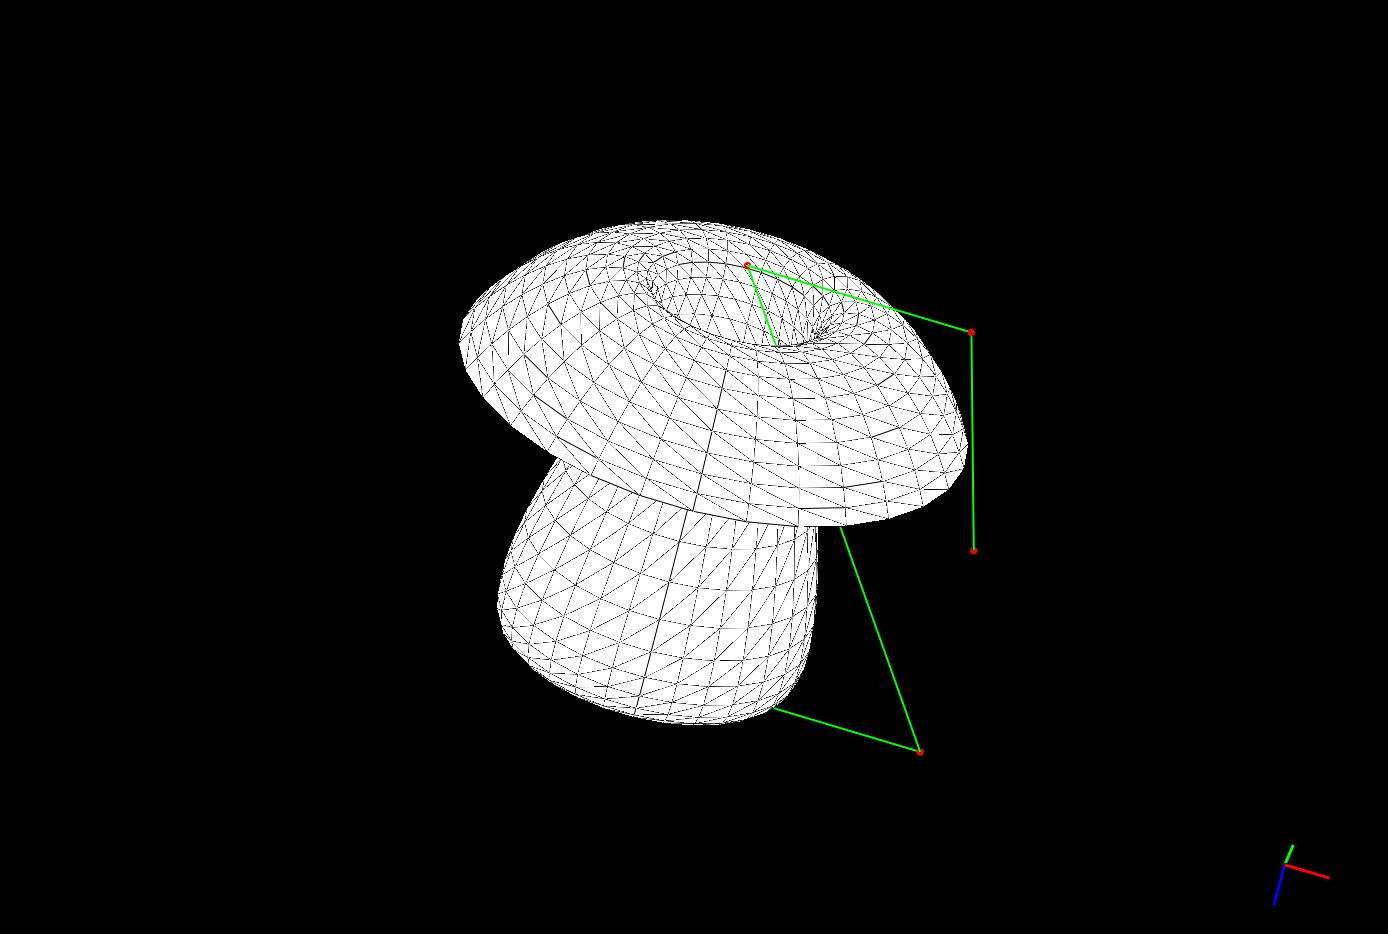
\includegraphics[scale=0.16]{img4}
\pagebreak

Освещение поверхности. Предусмотрено изменение всех парамертов материала (цвет, свойства материала воспринимать фоновое, рассеянное и зеркальное освещение, глянцевость), мощность фонового освещения и интенсивность точечного источника света.

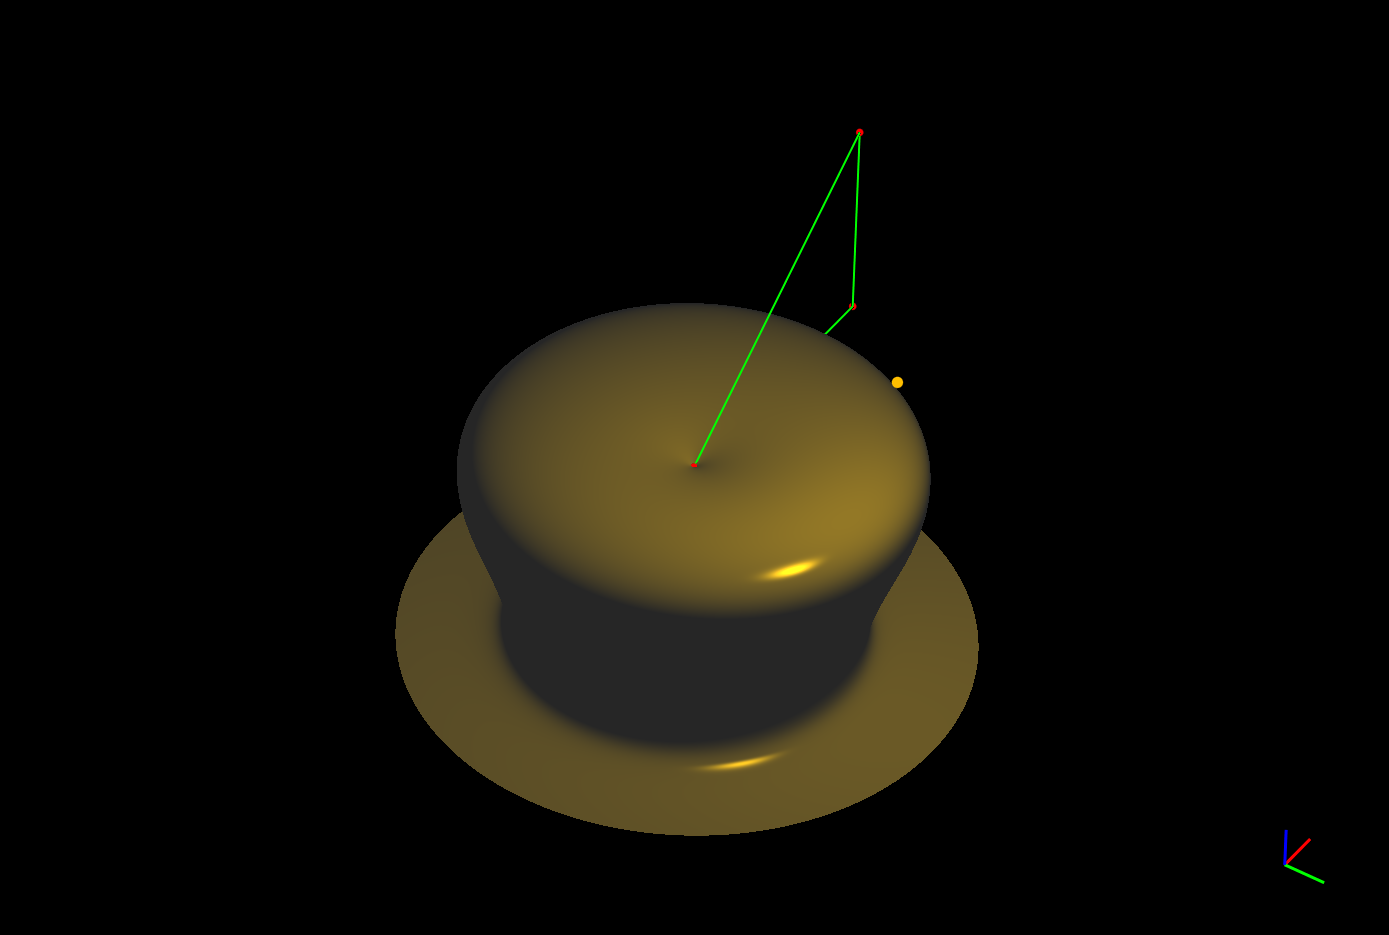
\includegraphics[scale=0.16]{img5}
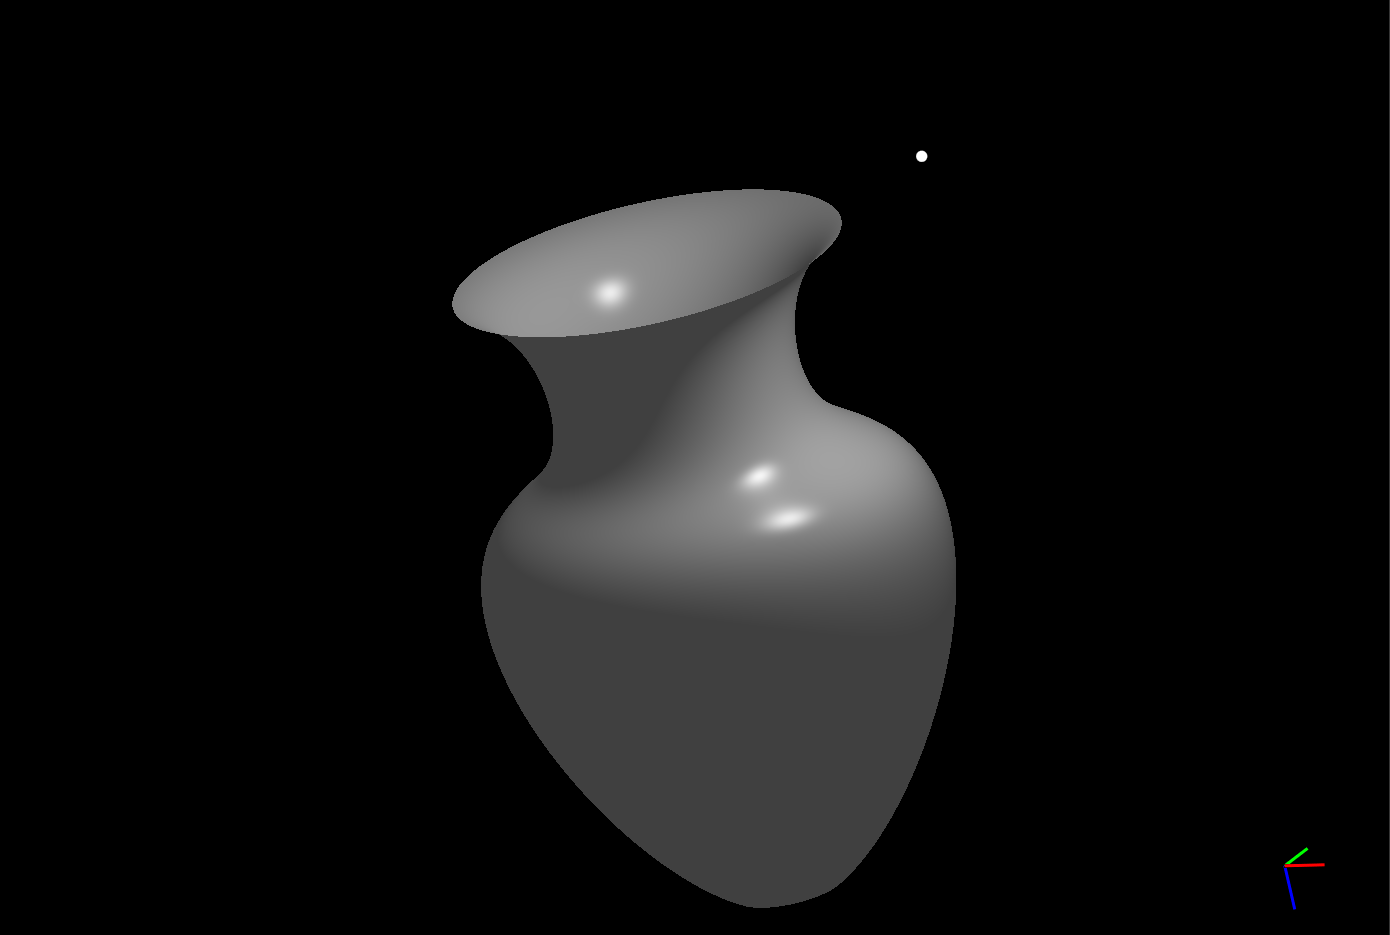
\includegraphics[scale=0.16]{img6}

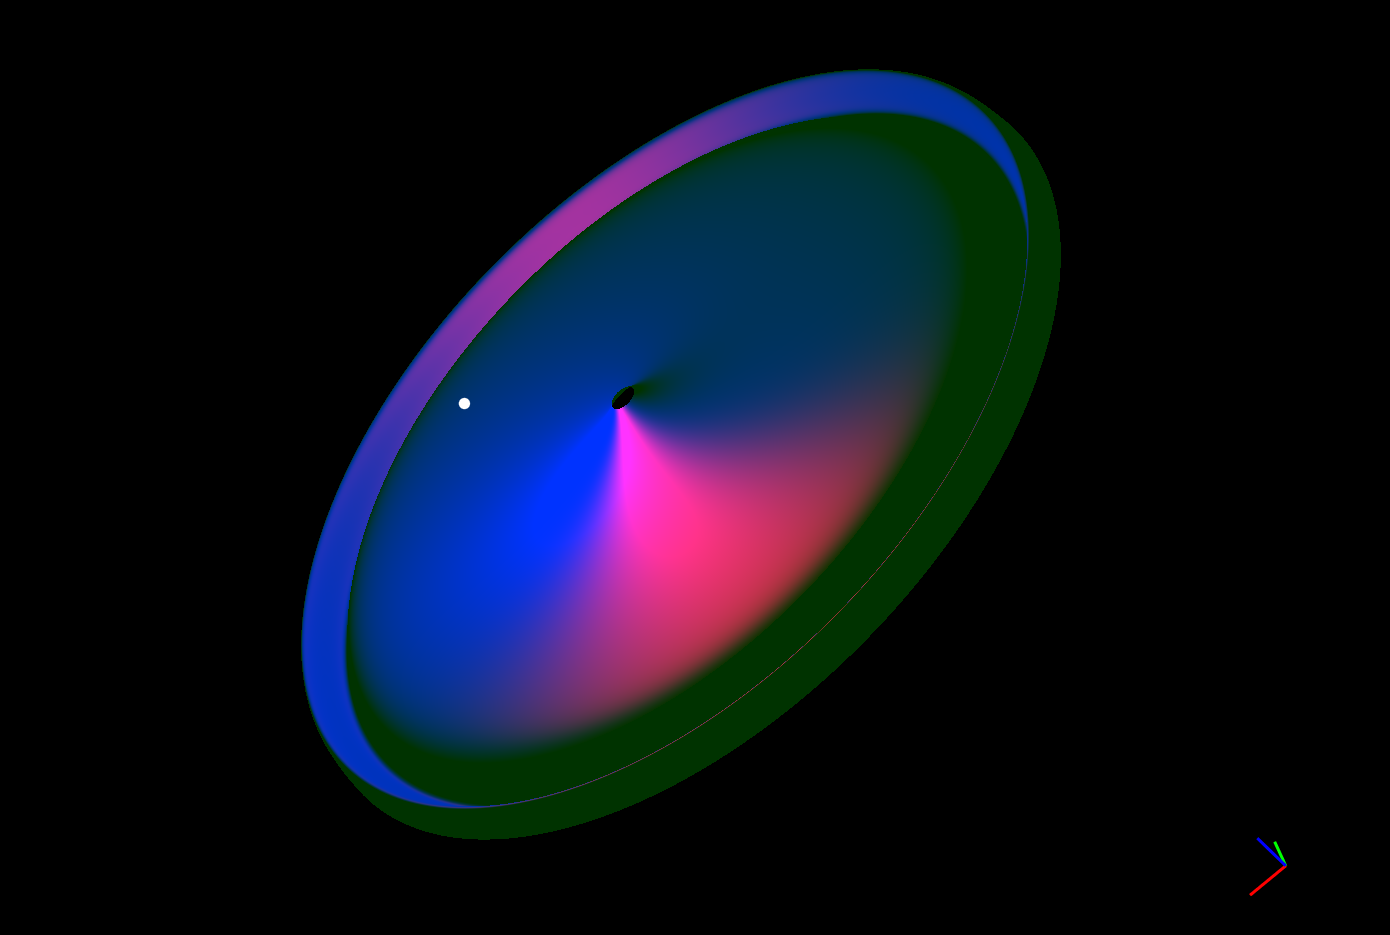
\includegraphics[scale=0.16]{img7}
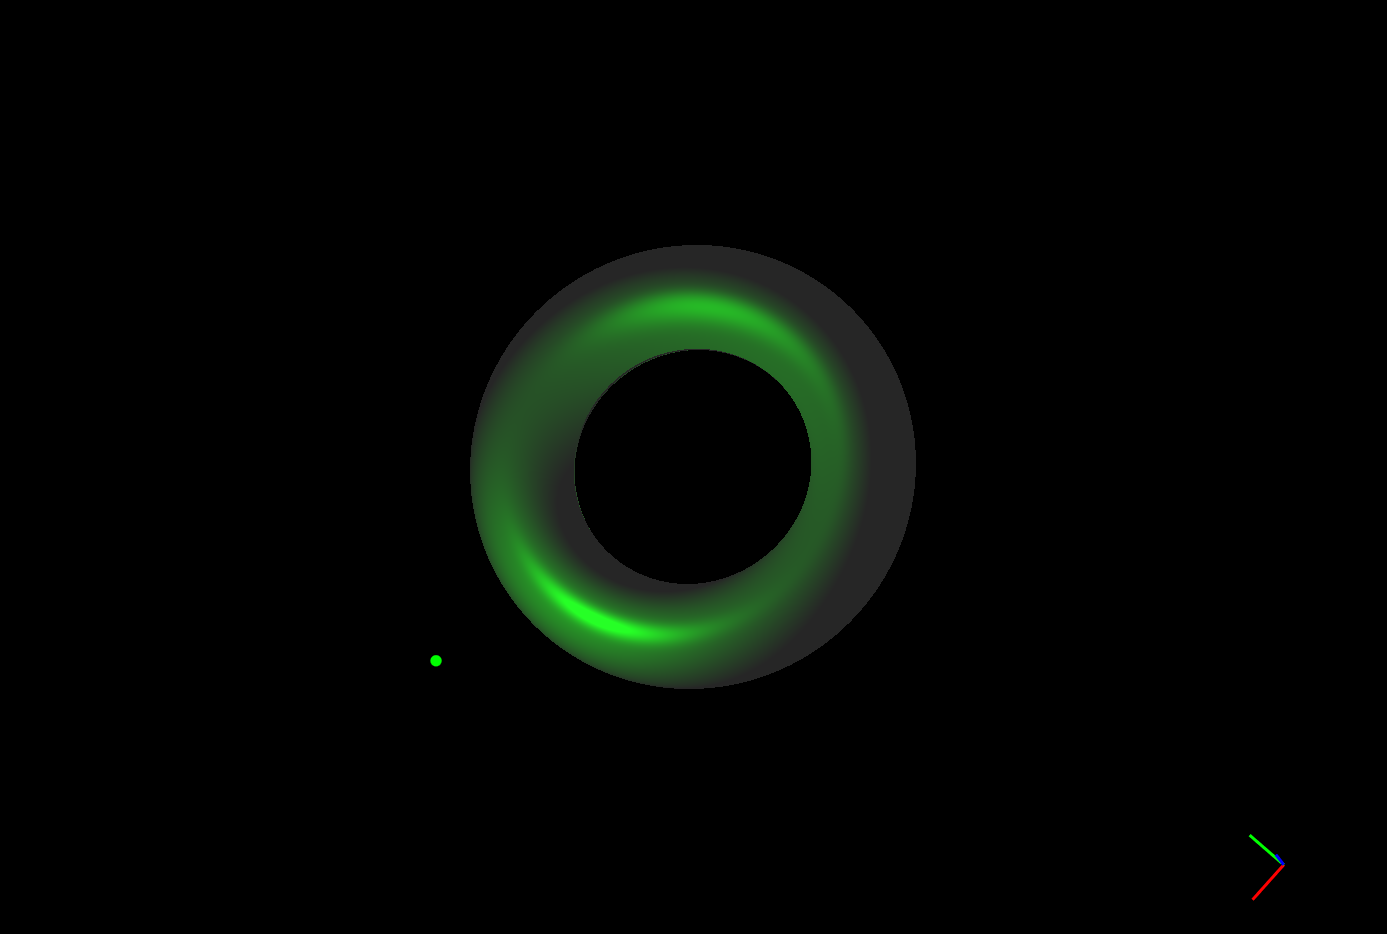
\includegraphics[scale=0.16]{img8}
\pagebreak
